\documentclass{article}


\usepackage{graphicx} % Required for inserting images
\usepackage{biblatex} %Imports biblatex package
\usepackage{booktabs} % Required for tables
\usepackage{longtable}
\usepackage{float}
\usepackage{rotating} % Required for sideways table

\addbibresource{references.bib}


\title{Learning to pump in slalom}
\author{Christian Magelssen}
\date{February 2024}


\begin{document}



\section{Introduction}
Elite athletes rely on effective strategies to continually enhance their skills and performance \cite{krakauer_motor_2019, taylor_role_2012, gray_plateaus_2017, tsay_strategy_2023}. In slalom skiing, these strategies aim to optimize the skier's navigation through a course, with the primary goal of achieving the shortest possible completion time. As long as skiers pass on the correct side of the gate marking the course, they are essentially free to choose any strategy they wish. Therefore, the number of strategies skiers can pick in any given situation is enormous, and they must learn to select the most appropriate strategy for each unique situation\cite{tsay_strategy_2023}. As such, coaches, athletes, and scientists have long searched for the best strategies that can contribute to executing the optimal turn in any given situation \cite{lemaster_skiers_1999, lemaster_ultimate_2010, reid_kinematic_2010, joubert_how_1967, joubert_ski_1978, luginbuhl_identification_2023, lind_physics_2013}. Since these strategies form the basis of all instruction on ski slopes (the what of learning), it is crucial to develop a firm understanding of which strategies may be effective. 

One course section of a slalom race where significant time differentials typically emerge, even in cases of equal finish times, is the flat sections\cite{supej_new_2011}. A defining characteristic of this terrain profile is that gravitational vector component pulling the skiers down the slope is small\cite{howe_new_2001}, which makes it key to  minimizing energy dissipation to maintain speed as much as possible \cite{supej_differential_2008}. Strategies that the skier can employ to achieve this goal include carving instead of skidding and regulate the fore/aft balance during a ski turn \cite{reid_turn_2009, reid_kinematic_2010}. 

A more offensive strategy is to increase the kinetic energy and thus the velocity through a turn by pumping \cite{lind_physics_2013}. According to Lind and Sanders' model \cite{lind_physics_2013}, skiers can enhance their kinetic rotational energy during a turn by shortening the radius of the axis around which they rotate. This can be achieved by skiers extending their center of mass, from a laterally inclined position, closer to this rotational axis (Fig. \ref{fig: design}b). Mechanically, this pushing motion effectively reduces the moment of inertia and consequently increases the skier's rotational kinetic energy, assuming conservation of angular momentum. In their model, the skier's gain in rotational kinetic energy from this motion is directly proportional to the amount of work exerted against the centrifugal force; thus, a larger extension movement results in a greater increase in rotational kinetic energy. Extending towards the axis of rotation can therefore potentially improve their skiing on flat terrain. 

Researchers have previously assumed that the contribution of pumping to increasing velocity through a turn is minimal and a negotiable mechanism to leverage to improve skiers' race times \cite{supej_differential_2008}. Critics argue that Lind and Sander's model neglects friction and that it should only work at low speeds \cite{supej_differential_2008, supej_how_2010}. Despite this, several studies have reported quantitative evidence that skilled alpine skiers gain additional kinetic energy at the exit of the turn—an increase that cannot be accounted for solely by their available potential energy at that moment \cite{reid_kinematic_2010, supej_differential_2008, supej_how_2010}. Thus, pumping appears to be a mechanism that skilled skiers already appears to exploit. Additionally, in a recent study, we provided evidence that skilled skiers massively improved their race times when they performed this extension movement \cite{magelssen_is_2022, christian_magelssen_reinforcement_2024}. In \cite{magelssen_is_2022}, the skiers' task were to navigate a course faster than by skiing straight down the hill. We used this task as a measure of whether skiers could increase their kinetic energy beyond the available amount of potential energy they have at the top, which would imply that skiing straight down would be the fastest. We reported that compared with straight-down gliding, the skiers significantly improved their time over the course of the training sessions. For three ski teams participating in the study, we monitored the skiers using a local positioning system before and after the intervention to gather their positional data as they traversed the sequence. In this paper, we investigate whether we can elucidate the improved race outcomes through kinematic analysis. 

\begin{figure}[H]
\centering
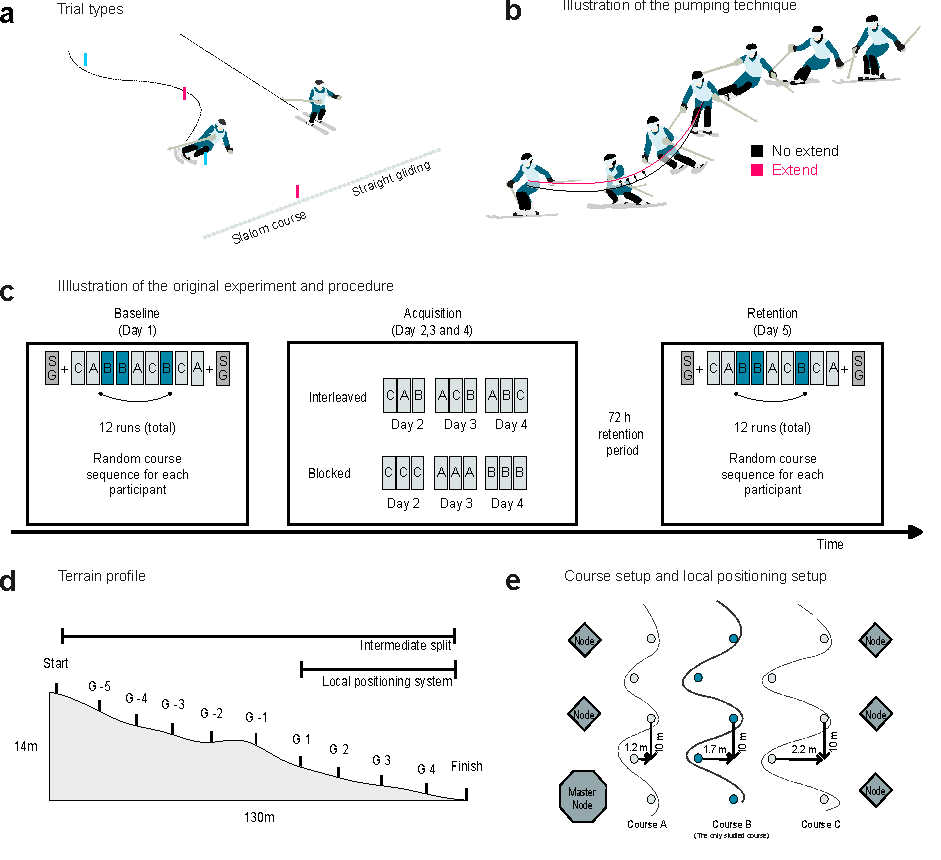
\includegraphics{figurer/figure_design.pdf}
\caption{Strategy selection for reinforcement learning (red) and supervised (free choice) learning (blue) during acquisition.}\label{fig: design}
\end{figure}


 


\section{Methods}


\subsection*{Participants}
The study's sample consisted of eighteen alpine ski racers (mean age = 16.7 years, SD = 1.1; 7 females, 11 males) from three development ski academies in Norway. These eighteen skiers formed a subset of a larger sample (64 skiers) from which we have already published results. We chose to subset this group because we only utilized a local positioning system at the upper section of the course for these skiers. With the exception of three participants, all had previously competed in Fédération Internationale de Ski (FIS) races, with FIS points recorded (mean = 115, SD = 31) in slalom. However, it is important to note that their FIS points may not accurately reflect their skill levels due to the challenges of organizing races during the COVID-19 pandemic, which limited opportunities to accumulate points.

\subsection{Setup}
The experiment took place on a 250-meter-long flat section of the race hill at SNØ, an indoor ski hall in Norway. Water was injected into this section before each ski team was tested to create an icy yet grippy snow layer. Three slalom courses (courses A, B, and C) were set over the section to investigate the contextual interference effect \cite{magelssen_is_2022}. The data reported in this study are only from Course B, which was set between courses A and C. Course B featured a 1.7-meter gate offset and a 10-meter vertical distance (blue course Fig. \ref{fig: design}e). This course was specifically selected for analysis because its dimensions are the most consistent with dimensions typical in a ski race.

A standardized starting procedure was used to minimize variation in entry speed. Skiers started 20 meters before the first gate from a stationary position with the forebinding positioned behind the start gate. Upon receiving clearance to start, skiers lifted their poles from the snow and skied straight down 10 meters from the hill until crossing the first photocell, which initiated the timer. Subsequently, skiers continued down the course. In this study, a trial concluded that when skiers crossed the second intermediate time, they continued skiing the rest of the course. The time data were recorded using a wireless photocell timing system (HC Timing wiNode and wiTimer; Oslo, Norway).

Within a smaller area of this section, a local positioning system (LPS) consisting of three nodes on each side of the track was deployed. One node acted as the master node and was situated on the skier's right side of the track. This LPS provided positional data as skiers descended from the course section (sampling frequency?). Using these data, the velocity and acceleration of the skiers were calculated. Initially, the plan was to track skiers using the LPS from start to finish. However, signal disruptions occurred in the upper part of the ski hall due to its narrow width, a common issue associated with LPS when nodes are positioned too close to walls. Consequently, the LPS data were filtered to focus solely on the sequence between the last five gates in the LPS section.

\subsection{Design and procedure}
The original study consisted of a five-day learning experiment with a three-day learning intervention involving pumping (Fig. \\ref{fig: design}c). On day 1, the skiers underwent a baseline test comprising a total of 9 runs (3 runs in each course), during which they received instructions solely to ski as quickly as possible down the courses and no timing as feedback. The runs were semirandomized to ensure that no more than two consecutive runs were conducted on the same course. Before and after the 9 runs in the slalom courses, the skiers performed a straight gliding (SG) run, where they descended the section straight down without any turns. Straight gliding (SG) was conducted in an upright, stationary posture to ensure a consistent drag area for each run (Fig.\ref{fig: design}a).

After the baseline test, all skiers gathered for a workshop where the principle of pumping was explained, and quantitative evidence of its effect was presented. Following this, the skiers were allocated into an interleaved group and a blocked learning group using a randomized blocked procedure. The interleaved group skied all slalom courses on the same day in an interleaved order, while the blocked group completed only one of the three courses per day (randomized and counterbalanced for each skier). Skiers in both groups received race times as feedback after each trial, expressed as the difference between course time and straight gliding run time. Further specifics of the experiment and procedure can be found in the original study \cite{magelssen_is_2022}. Since evidence for the contextual interference effect was not found in this study, we omitted this group information in the modeling work and henceforth only described the procedure.

After the three acquisition sessions (days 2, 3, and 4), the skiers had a break during which they did not ski. Following this break, skiers underwent a retention test (similar to baseline) consisting of a total of 9 runs (3 runs in each course). During this test, they received instructions to ski as quickly as possible down the courses, with no timing provided as feedback, similar to the baseline procedure.


\subsection{Analysis}
The cleaning and processing of the data began with custom functions in MATLAB, which were developed, tested, and utilized in previous studies \cite{reidKinematicKineticStudy2010}. Subsequently, the files were imported into Python using the \cite{2020SciPy-NMeth} and pandas \cite{reback2020pandas} packages. During this import, some runs caused import problems in Python because they were not part of the experimental protocol (warm-up runs or freeski runs).
Additionally, in a few cases, the quality of the local positioning signal was deficient, preventing the calculations in MATLAB from proceeding. In both error cases, we manually removed the runs from the MATLAB file. After this processing step, the remaining data underwent two manual screening processes to verify the quality of the local positioning data. The first screening process involved removing all runs that did not match the experimental procedure, such as warm-up runs or runs where a Did Not Finish (DNF) was recorded. In the second screening process, all runs were visually inspected to identify errors in the local positioning data. To aid in this detection, the section time performance, coordinates, and velocity for all ski racers were plotted. All removed runs, along with the reasons for their removal, are documented in document A. Finally, the data that passed the screening process was saved as a .csv file. An extensive report of this cleaning and validation process can be found at OSF  (\url{https://osf.io/2jxgk}).

Our general statistical approach was to leverage multilevel modeling due to the hierarchical data structure of our data. This structure stemmed from two sources: repeated observations in each slalom course on baseline and retention, and the nesting of skiers within different ski academies that conducted the learning experiment together. We employed a Bayesian estimation approach as our goal was to describe the change and its effects rather than testing \cite{kruschke_bayesian_2018}. To fit the model, we used the brms \cite{burkner_brms_2017} package in R \cite{r_core_team_r_2022}. To extract and visualize draws from the model we used Tidybayes package \cite{kay_tidybayes_nodate}. 

With the exception of one model, we employed multilevel Generalized Additive Models (GAMs) for all our analyses. GAMs model the global trend using smooth functions composed of several simple basis functions, each with an estimated coefficient derived from the data. The estimated relationship between the predictor and the response is obtained by summing up the coefficients of the total number of basis functions supported by the data. Adding many basis functions allows for modeling more complex shapes but may lead to overfitting the data. However, the GAM framework counteracts this issue of overly complex models by penalizing the coefficients of the basis functions, effectively negotiating the tradeoff between wiggly functions and generalizability.


\subsection{Race times}
To analyze the race times, we conducted two statistical analyses. In the first model, we examined the time it took from the start to the first intermediate time, which was positioned just after the finish of the LPS section (Fig. \ref{fig: design}d). In this model, we predicted Race time (measured as time behind straight gliding in the respective session), with Session (baseline, retention) as fixed effect, and a random intercept and slope for skiers. Due to the limited number of levels in the ski group, we were unable to achieve model convergence with ski group as a varying intercept or slope. We used an index coding approach for both analyses, which uses integers (1, 2, ..., n) to code categorical variable levels. The advantage of this approach over traditional treatment coding is that it avoids placing more equal uncertainty on all levels of that variable as opposed to treatment coding, which assigns more uncertainty to all levels other than the reference group. With the Bayesian modeling approach, it is also easier to set sensible priors \cite{mcelreath_statistical_2018}. 

For the second model, we used position data from the local positioning system (LPS). These data were normalized to ensure an equal number of data points between the gates in the sequence. To model the race times, we employed the difference between the time in the course and the time straight down for the entire sequence. We modeled this difference with a multilevel generalized additive model (GAM) as a global smooth plus group-level smoothers (random smooth) for each skier \cite{pedersen_hierarchical_2019}. We opted for group-level smoothers because we know that kinematic data can vary significantly between skiers.



\section{Results}



\subsection{Race time}
We analyzed the skiers' race time from the section's start to its end (intermediate split) and the race time in the section covered by the local position system (LPS section). This analysis aimed to ensure that the skiers also improved in the top section of the slalom course, providing a basis for further kinematic analysis to explain this improvement. Our analysis revealed that, on average, the skiers improved their race time by -0.17 sec. (95\% Credible intervals (CI)[-0.33, 0.01]) from the baseline to the retention session on the entire section. Zooming into the LPS section, we found that, on average, the skiers improved their race time by -0.1 sec. (95\% CI[-0.1, -0.09]). Thus, we identified this section as important for further analysis. Fig. \ref{fig: choice_estimated} shows the estimated race times for baseline and retention and their differences for the two analyzed sections. 

\begin{figure}[H]
\centering
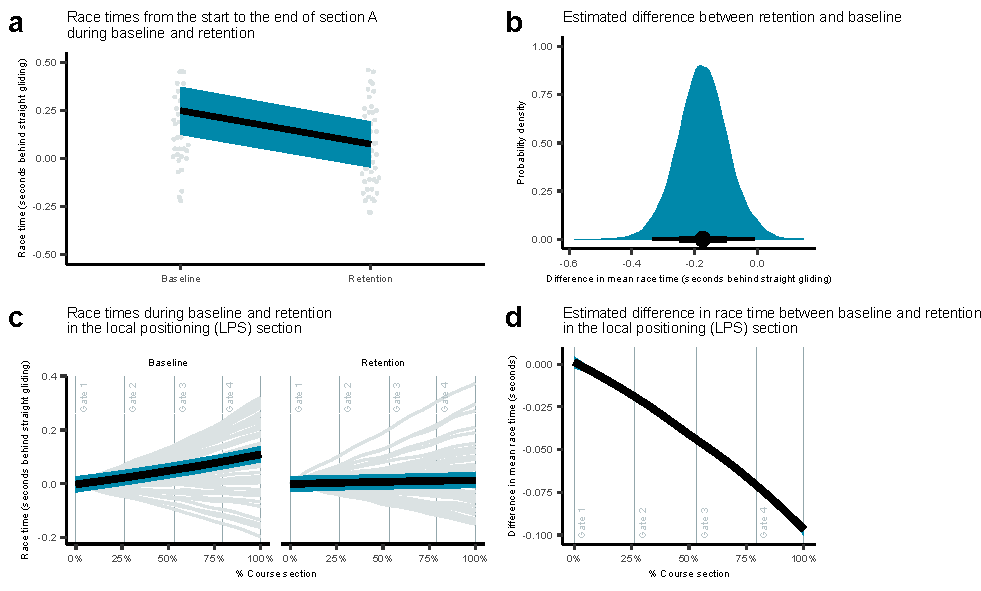
\includegraphics{figurer/figure_racetime_2.pdf}
\caption{Strategy selection for reinforcement learning (red) and supervised (free choice) learning (blue) during acquisition.}\label{fig: choice_estimated}
\end{figure}

\subsection{Velocity}
We chose to study the kinematic changes among the skiers in this section, as we observed time differences between baseline and retention. If the skiers' extension motion towards the axis of rotation of the turn increases velocity, we would expect an increased velocity close or immediately after the turn. Figure \ref{fig: velocity}a depicts the velocity profiles for the section with the local positioning system (LPS) at baseline and retention.  

Before the intervention (baseline), the skiers' velocity decreased on average by -0.14 (95\% CI [-0.36, 0.09]) from gate 1 to 4 in the sequence. After the training intervention, skiers increased their entry velocity into the section by an average of 0.24 m/s (95\% CI [0.19, 0.29]) compared to the velocity during the baseline. The velocity continued to increase through the sequence, rising on average by 0.16 m/s (95\% CI [0.10, 0.21]) from gate 1 to gate 4. Not only did the skiers increase their velocity throughout the section—almost incrementally from gate to gate—but the velocity profile also underwent a change with significantly more waveforms. In general, the pattern of these waveforms was that skiers increased their velocity after gate passage and continued to rise until the skier was between two gates. After that, the velocity decreased to gate passage before it rose again. 

Selv om vi ikke kan si noe sikkert kan det se ut som at skikjørerende pumpet seg opp i høyere hastighet gjennom sekvensen









\begin{figure}[H]
\centering
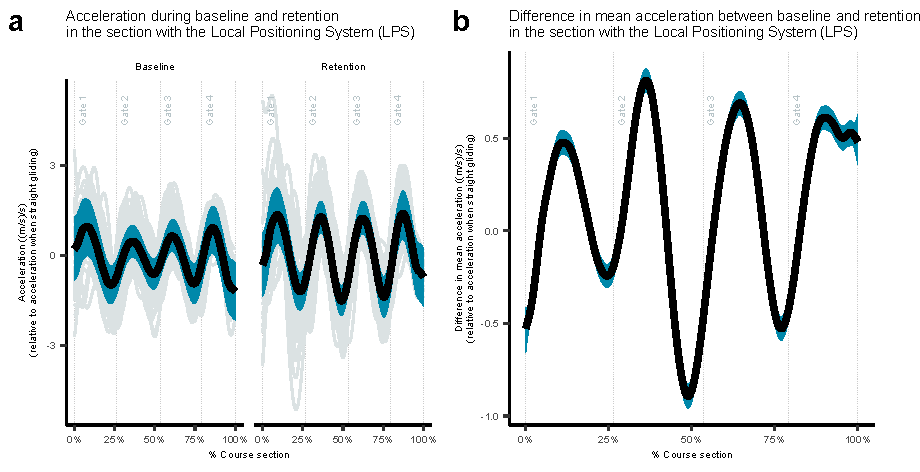
\includegraphics{figurer/figure_acc.pdf}
\caption{Strategy selection for reinforcement learning (red) and supervised (free choice) learning (blue) during acquisition.}\label{fig: choice_estimated}
\end{figure}

































We chose to study the kinematic changes among the skiers in this section, as we observed time differences between baseline and retention. Om skikjørernes strekkbevegelse mot svingens axis of rotation fra lateralt innoverlent posisjon øker hastigheten vil vi forvente en økt hastighet rett etter svingen. Figure \ref{fig: velocity}a displays the velocity profiles for the LPS section at baseline and retention. During baseline, velocity declined relative to the velocity when straight gliding (From gate 1 to gate 4, the velocity decreased by -0.14 m/s (95\% CI [-0.36, 0.09]).


The third strategy that can potentially make skiers faster on flat slopes in slalom is to 'extend,' also referred to as 'pumping' to increase velocity \cite{lind_physics_2013}. By moving closer to the axis of rotation of a turn from a laterally inclined position, the skier can boost its kinetic rotational energy under certain situations. According to Lind and Sanders \cite{lind_physics_2013} model, the skier achieves this effect by shortening the radius of the axis about which they rotate, which will reduce the moment of inertia and consequently increase the rotational kinetic energy of the system under the assumption that angular momentum is conserved. In their model, the gain in rotational kinetic energy from this motion is proportional to the amount of work the skier does against the centrifugal force; therefore, a larger extension movement will accomplish a greater increase in rotational kinetic energy.



Vi forventet at skikjørernes forbedrede tider skyltes 



A key explanation behind the improvement in skiers through the LPS-section was that they pumped themselves to higher velocities. Consistent with pumping contributing to a velocity increase after its execution, we predicted that a large velocity increase around the gate passage, caused by the intervention.

Figure \ref{fig: velocity}a displays the velocity profiles for the LPS section at baseline and retention. During baseline, velocity declined relative to the velocity when straight gliding (From gate 1 to gate 4, the velocity decreased by -0.14 m/s (95\% CI [-0.36, 0.09]).

After the intervention, we observed a large change in the velocity profile (Figure \ref{fig: velocity}b). We found that skiers had a higher entry velocity at retention. The expected average difference was 0.24 (95\% CI [0.19, 0.29]) at the first gate in the section. However, we also identified a global trend indicating that skiers continued to increase their velocity throughout the section. The expected difference in increase from gate 1 to gate 4 was 0.16 m/s (95\% CI [0.10, 0.21]).

Den tydeligste endringen var likevel rett etter porten. Etter intervensjonen var hastighetsprofilen betydelig mer bølgeformet med store. Den forventede økningen mellom


\begin{figure}[H]
\centering
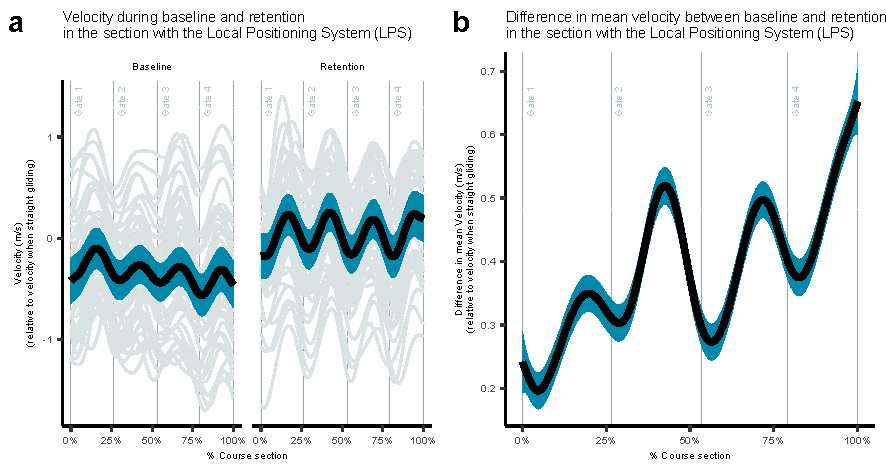
\includegraphics{figurer/figure_velocity_2.pdf}
\caption{Strategy selection for reinforcement learning (red) and supervised (free choice) learning (blue) during acquisition.}\label{fig: velocity}
\end{figure}








\printbibliography %Prints bibliography

\end{document}
